\chapter{THEORETICAL BASIS}

\renewcommand{\headrulewidth}{0.5pt}
\renewcommand{\footrulewidth}{0.5pt}
\thispagestyle{plain}
\pagestyle{fancy}
\fancyhf{}
\fancyhead[L]{\textbf{CHAPTER 2}}
\fancyhead[R]{\textbf{DANGEGOUS WEAPONS DETECTION USING YOLOv9}}
\raggedright
\fancyfoot[L]{From: Nguyen Van Anh Tuan}
\fancyfoot[R]{Page \thepage}

\justifying

\section{Overview about YOLOv9}
    \begin{figure}[H]
        \centering
        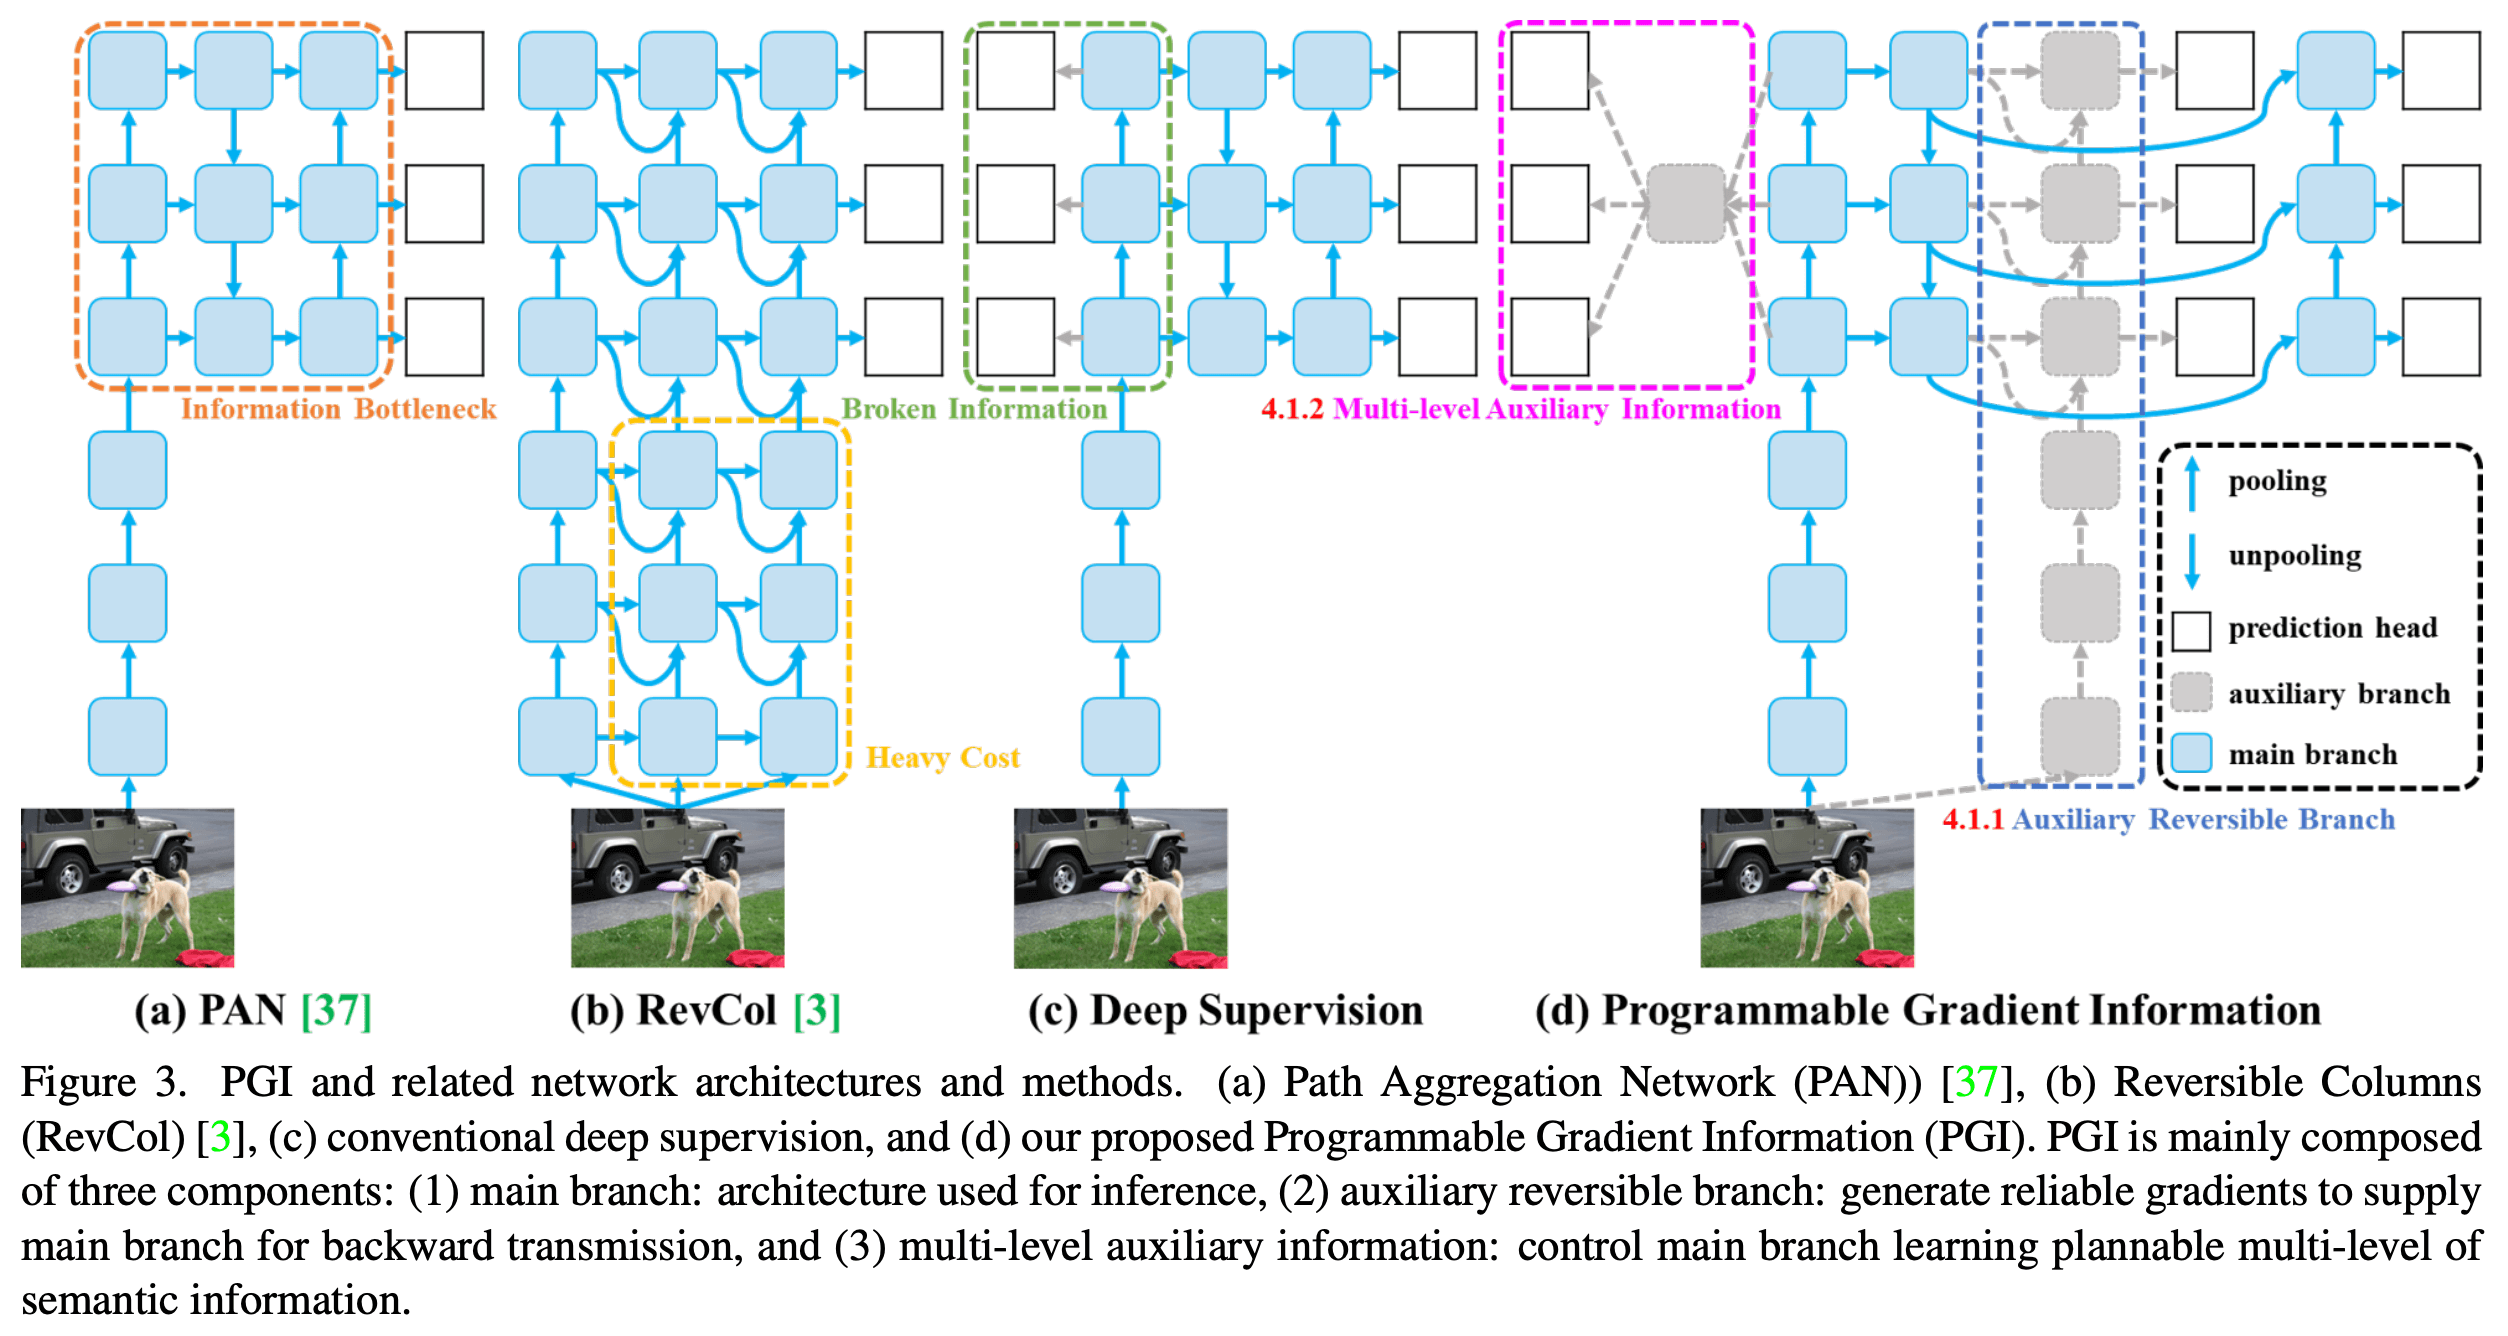
\includegraphics[width=0.8\linewidth]{img/core_innovation.png}
        \caption{PGI and related network architectures and methods. }\
        \label{fig:PGI}
    \end{figure}
    With the continuous evolution of computer vision technologies, YOLOv9 emerges as the latest advancement, developed by Chien-Yao
    Wang, I-Hau Yeh, and Hong-Yuan Mark Liao. This trio of researchers has a rich history in the field, having contributed to the
    development of preceding models such as YOLOv4, YOLOR, and YOLOv7. \\
    \begin{figure}[H]
        \centering
        
\includegraphics[width=0.8\linewidth]{img/ultralytics.jpg}
        \caption{Ultralytics's logo}
    \end{figure}
    YOLOv9 marks a significant advancement in real-time object detection, introducing groundbreaking techniques such as Programmable
    Gradient Information (PGI) and the Generalized Efficient Layer Aggregation Network (GELAN). This model demonstrates remarkable
    improvements in efficiency, accuracy, and adaptability, setting new benchmarks on the MS COCO dataset. \\
    \begin{figure}[H]
        \centering
        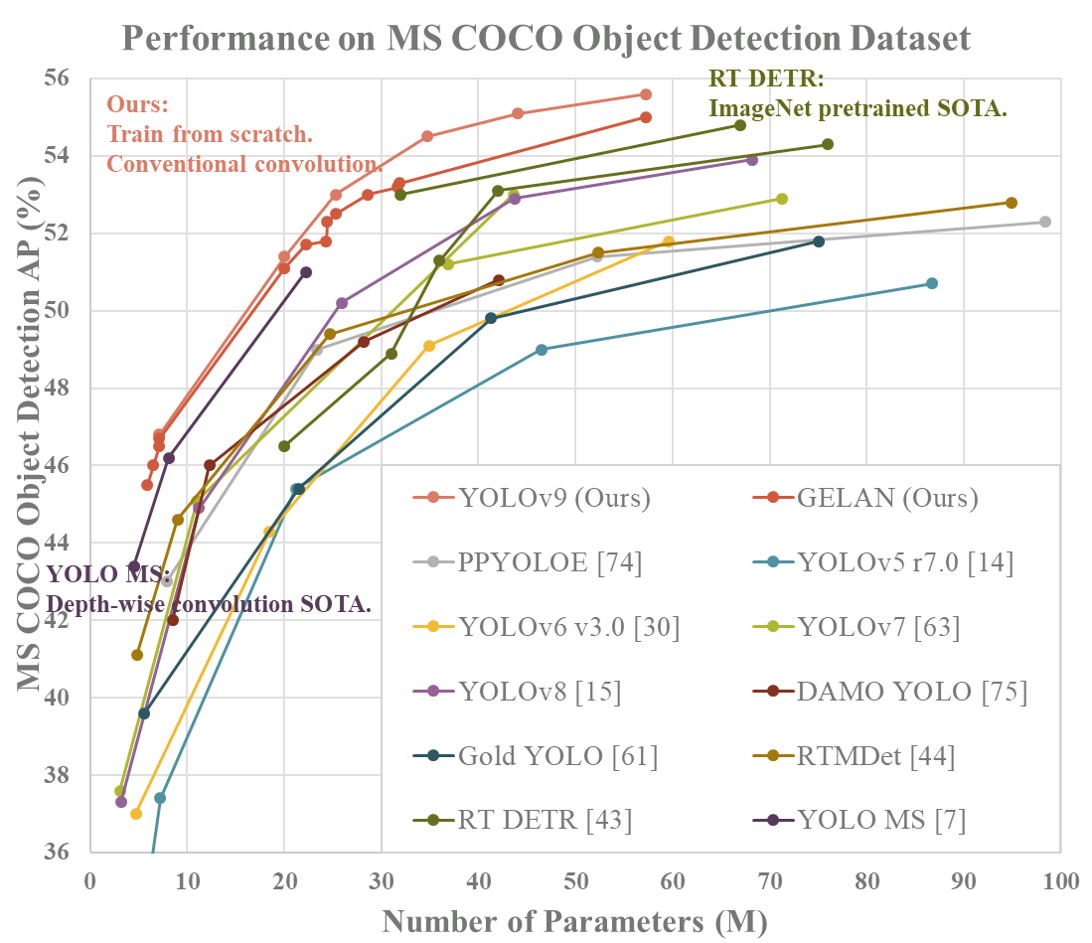
\includegraphics[width=0.8\linewidth]{img/performance_yolov9.png}
        \caption{Comparisons of the real-time object detecors on MS COCO dataset}
    \end{figure}
    In the quest for optimal real-time object detection, YOLOv9 stands out with its innovative approach to overcoming information loss
    challenges inherent in deep neural networks. By integrating PGI and the versatile GELAN architecture, YOLOv9 not only enhances the
    model's learning capacity but also ensures the retention of crucial information throughout the detection process, thereby achieving
    exceptional accuracy and performance.

\section{Methodology}
    \subsection{Programmable Gradient Information (PGI)}
        In order to solve the aforementioned problems, it was proposed 
        a new auxiliary supervision framework called Programmable 
        Gradient Information (PGI), as shown in Figure \ref{fig:PGI}.
        PGI mainly includes three components, namely
        (1) main branch, (2) auxiliary reversible branch, and (3)
        multi-level auxiliary information. From Figure \ref{fig:PGI} we
        see that the inference process of PGI only uses main branch
        and therefore does not require any additional inference cost.
        As for the other two components, they are used to solve or
        slow down several important issues in deep learning methods. 
        Among them, auxiliary reversible branch is designed
        to deal with the problems caused by the deepening of neural
        networks. Network deepening will cause information bottleneck, 
        which will make the loss function unable to generate reliable
        gradients. As for multi-level auxiliary information, it is designed
        to handle the error accumulation problem
        caused by deep supervision, especially for the architecture
        and lightweight model of multiple prediction branch. Next,
        we will introduce these two components step by step
        \subsubsection{Auxiliary Reversible Branch}
            In PGI, it was proposed auxiliary reversible branch to generate 
            reliable gradients and update network parameters. By
            providing information that maps from data to targets, the
            loss function can provide guidance and avoid the possibility 
            of finding false correlations from incomplete feed forward 
            features that are less relevant to the target. We propose
             the maintenance of complete information by introducing
             reversible architecture, but adding main branch to reversible
             architecture will consume a lot of inference costs.
            We analyzed the architecture of \ref{fig:PGI} and found that
            when additional connections from deep to shallow layers
            are added, the inference time will increase by 20\%. When
            we repeatedly add the input data to the high-resolution computing
            layer of the network (yellow box), the inference time
            even exceeds twice the time.
            \begin{figure}[H]
                \centering
                \includegraphics[width=0.8\linewidth]{img/GELAN.png}
                \caption{The architecture of GELAN: (a) CSPNet [64], (b) ELAN [65], and (c) proposed GELAN. We imitate CSPNet and extend ELAN into GELAN that can support any computational blocks}
                \label{fig:GELAN}
            \end{figure}
            Finally, since auxiliary reversible branch can be removed
            during the inference phase, the inference capabilities of the
            original network can be retained. We can also choose any
            reversible architectures in PGI to play the role of auxiliary
            reversible branch
        \subsubsection{Multi-level Auxiliary Information}
            In this section we will discuss how multi-level auxiliary in-
            formation works. The deep supervision architecture includ-
            ing multiple prediction branch is shown in \ref{fig:PGI}. For
            object detection, different feature pyramids can be used to
            perform different tasks, for example together they can de-
            tect objects of different sizes. Therefore, after connecting
            to the deep supervision branch, the shallow features will be
            guided to learn the features required for small object detec-
            tion, and at this time the system will regard the positions
            of objects of other sizes as the background. However, the
            above deed will cause the deep feature pyramids to lose a lot
            of information needed to predict the target object. Regard-
            ing this issue, we believe that each feature pyramid needs
            to receive information about all target objects so that subse-
            quent main branch can retain complete information to learn
            predictions for various targets.\\
            \vspace{3mm}
            The concept of multi-level auxiliary information is to in-sert
            an integration network between the feature pyramid hi-
            erarchy layers of auxiliary supervision and the main branch,
            and then uses it to combine returned gradients from differ-
            ent prediction heads, as shown in Figure 3 (d). Multi-level
            auxiliary information is then to aggregate the gradient infor-
            mation containing all target objects, and pass it to the main
            branch and then update parameters. At this time, the charac-
            teristics of the main branch’s feature pyramid hierarchy will
            not be dominated by some specific object’s information. As
            a result, our method can alleviate the broken information
            problem in deep supervision. In addition, any integrated
            network can be used in multi-level auxiliary information.
            Therefore, plan the required semantic levels to guide
            the learning of network architectures of different sizes.
    \subsection{Generalized Efficient Layer Aggregation Network (GELAN)}
        \subsubsection{Generalized ELAN}
            For GELAN, first do ablation studies for computational
            blocks. Used Res blocks [21], Dark blocks [49], and
            CSP blocks [64] to conduct experiments, respectively. \ref{tab:GELAN}
            shows that after replacing convolutional layers in
            ELAN with different computational blocks, the system can
            maintain good performance. Users are indeed free to re-
            place computational blocks and use them on their respective
            inference devices. Among different computational block re-
            placements, CSP blocks perform particularly well. They
            not only reduce the amount of parameters and computation,
            but also improve AP by 0.7\%. Therefore, choose CSP-
            ELAN as the component unit of GELAN in YOLOv9. \\
            \begin{table}[ht]
                \centering
                \begin{tabular}{| l | l | l | l | l |}
                    \hline
                    \rowcolor{lightgray} Model & CB type & \#Param. & FLOPs & AP${^{val}_{50:95}}$ \\ \hline
                    GELAN-S & Conv & 6.2M & 23.5G & 44.8\% \\ \hline
                    GELAN-S & Res [21] & 5.4M & 21.0G & 44.3\% \\ \hline
                    GELAN-S & Dark [49] & 5.7M & 21.8G & 44.5\% \\ \hline
                    GELAN-S & CSP [64] & 5.9M & 22.4G & 45.5\% \\ \hline
                \end{tabular}
                \caption{Ablation study on various computational blocks}
                \label{tab:GELAN}
            \end{table}
            Next, conduct ELAN block-depth and CSP block-
            depth experiments on GELAN of different sizes, and display
            the results in \ref{tab:ELAN-CSP}. We can see that when the depth
            of ELAN is increased from 1 to 2, the accuracy is significantly
            improved. But when the depth is greater than or
            equal to 2, no matter it is improving the ELAN depth or the
            CSP depth, the number of parameters, the amount of computation,
            and the accuracy will always show a linear relationship.
            This means GELAN is not sensitive to the depth.
            In other words, users can arbitrarily combine the components
            in GELAN to design the network architecture, and
            have a model with stable performance without special design.
            In \ref{tab:ELAN-CSP}, for YOLOv9-{S,M,C}, set the pairing
            of the ELAN depth and the CSP depth to {{2, 3}, {2, 1},
            {2, 1}}. \\
            \vspace{3mm}
            GELAN represents a strategic architectural advancement, enabling YOLOv9 to achieve superior parameter utilization and computational efficiency. Its design allows for flexible integration of various computational blocks, making YOLOv9 adaptable to a wide range of applications without sacrificing speed or accuracy.
            \begin{table}[ht]
                \centering
                \begin{tabular}{| l | l | l | l | l | l |}
                    \hline
                    \rowcolor{lightgray} Model & $D_{ELAN}$ & $D_{CSP}$ & \#Param. & FLOPs & AP${^{val}_{50:95}}$ \\ \hline
                    GELAN-S & 2 & 1 & 5.9M & 22.4G & 45.5\% \\ 
                    GELAN-S & 2 & 2 & 6.5M & 24.4G & 46.0\% \\ 
                    GELAN-S & 3 & 1 & 7.1M & 26.3G & 46.5\% \\ 
                    GELAN-S & 2 & 3 & 7.1M & 26.4G & 46.7\% \\ \hline
                    GELAN-M & 2 & 1 & 20.0M & 76.3G & 51.1\% \\ 
                    GELAN-M & 2 & 2 & 22.2M & 85.1G & 51.7\% \\ 
                    GELAN-M & 3 & 1 & 24.3M & 93.5G & 51.8\% \\ 
                    GELAN-M & 2 & 3 & 24.4M & 94.0G & 52.3\% \\ \hline
                    GELAN-C & 1 & 1 & 18.9M & 76.3G & 51.1\% \\ 
                    GELAN-C & 2 & 1 & 25.3M & 85.1G & 51.7\% \\ 
                    GELAN-C & 2 & 2 & 28.6M & 93.5G & 51.8\% \\
                    GELAN-C & 3 & 1 & 31.7M & 93.5G & 51.8\% \\
                    GELAN-C & 2 & 3 & 31.9M & 94.0G & 52.3\% \\ \hline
                \end{tabular}
                \caption{Ablation study on ELAN and CSP depth}
                \label{tab:ELAN-CSP}
            \end{table}
            \begin{figure}[H]
                \centering
                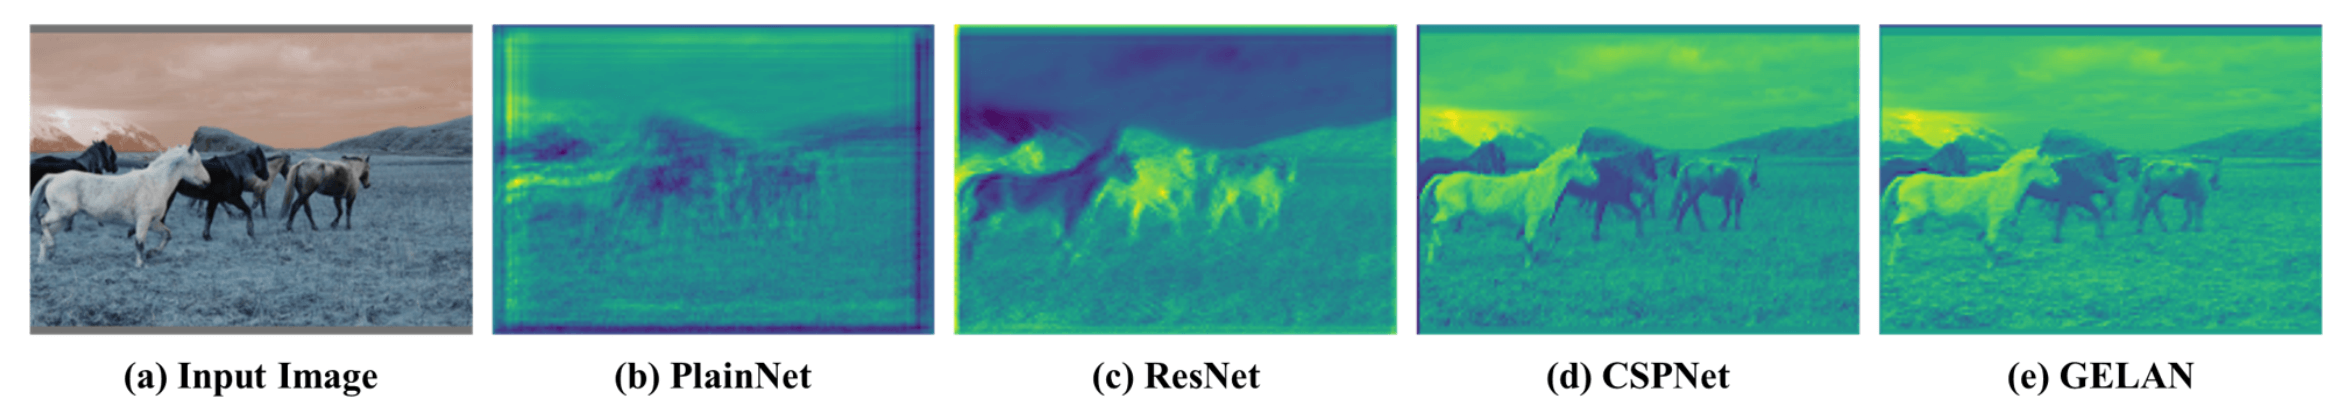
\includegraphics[width=0.8\linewidth]{img/gelan.png}
                \caption{Visualization results of random initial weight output feature maps for different network architectures: (a) input image, (b)PlainNet, (c) ResNet, (d) CSPNet, and (e) proposed GELAN. From the figure, we can see that in different architectures, the information provided to the objective function to calculate the loss is lost to varying degrees, and our architecture can retain the most complete information and provide the most reliable gradient information for calculating the objective function.}
                \label{fig:gelan}
            \end{figure}
    \subsection{Implimentation Details}
        \begin{figure}[H]
            \centering
            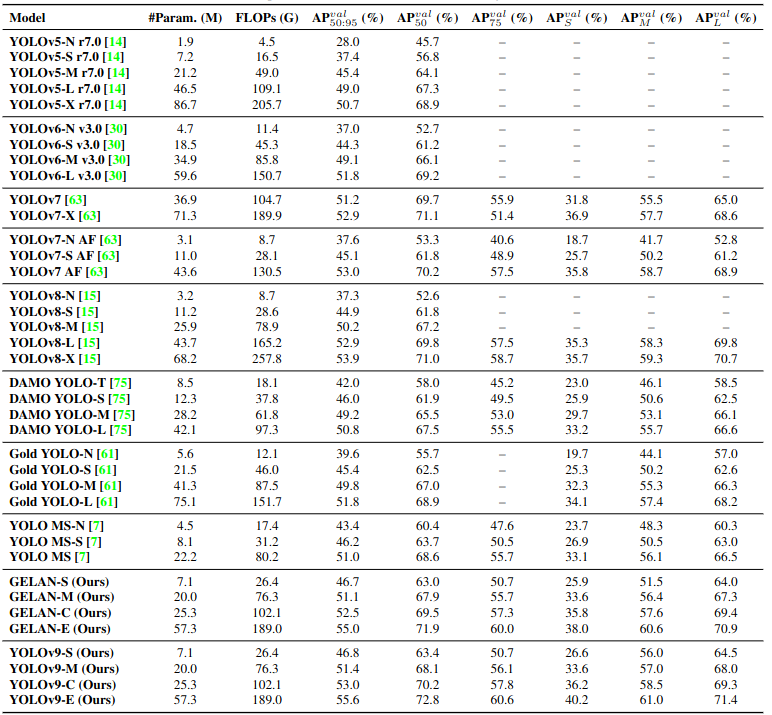
\includegraphics[width=0.9\linewidth]{img/comparison.png}
            \caption{Comparison of state-of-the-art real-time object detectors}
            \label{fig:comparison}
        \end{figure}
        \begin{figure}[H]
            \centering
            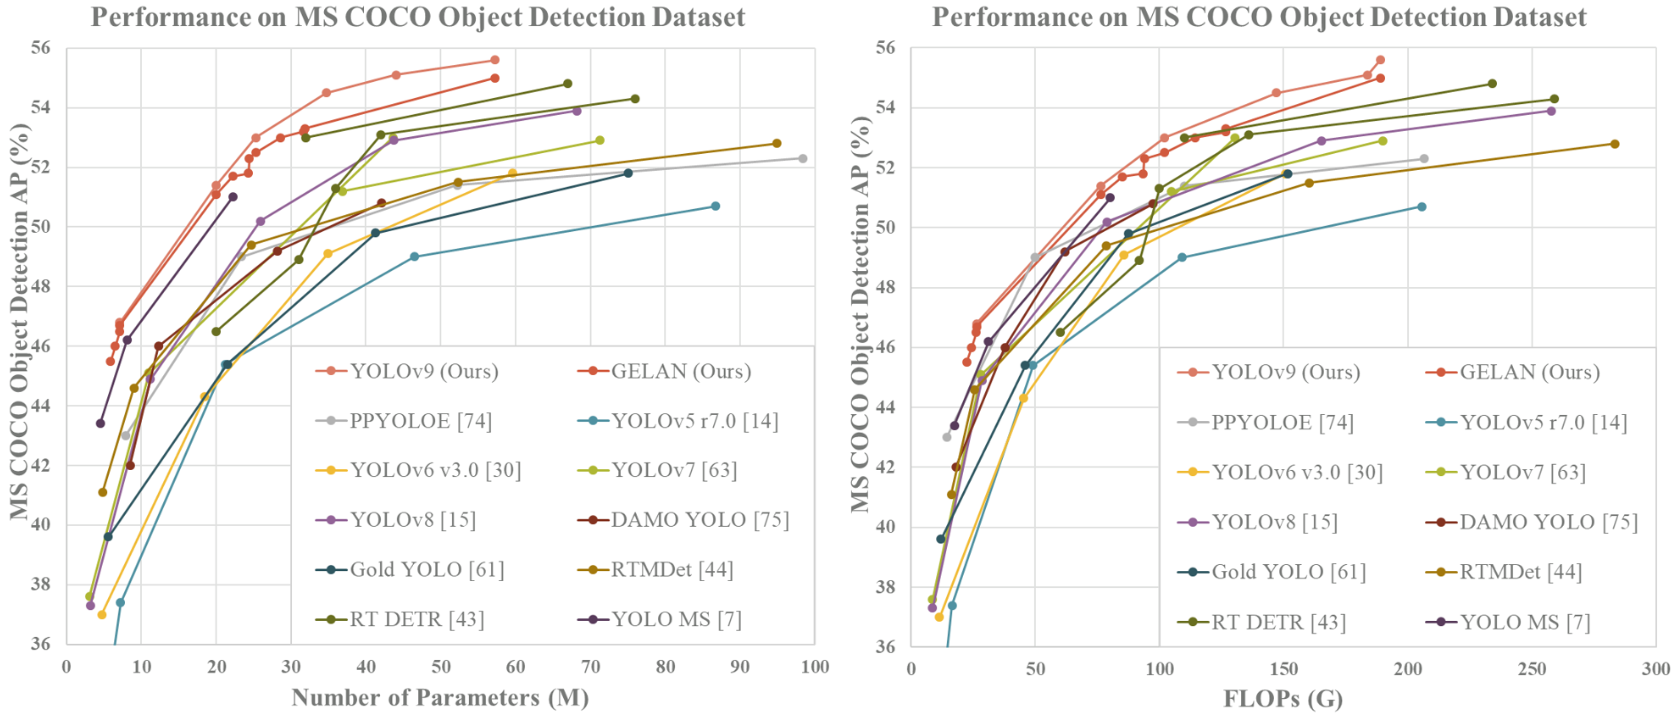
\includegraphics[width=0.9\linewidth]{img/tate-of-the-art_real-time.png}
            \caption{Comparison of state-of-the-art real-time object detectors. The methods participating in the comparison all use ImageNet as pre-trained weights, including RT DETR [43], RTMDet [44], and PP-YOLOE [74], etc. The YOLOv9 that uses train-from-scratch method clearly surpasses the performance of other methods.}
            \label{fig:state-of-the-art}
        \end{figure}

\section{Python Programming Language}
    \subsection{Introduce About Python Programming Language}
        \begin{figure}[H]
            \centering
            
\includegraphics[width=0.8\linewidth]{img/python-logo.jpg}
            \caption{Python Programming Language}
            \label{fig:python}
        \end{figure}
        Python is an interpreted high-level general-purpose programming language. Python's design philosophy emphasizes code readability 
        with its notable use of significant indentation. Its language constructs as well as its object-oriented approach aim to help programmers 
        write clear, logical code for small and large-scale projects. \\
        \vspace{3mm}
        Python is dynamically-typed and garbage-collected. It supports multiple programming paradigms, including structured (particularly, procedural), 
        object-oriented and functional programming. Python is often described as a "batteries included" language due to its comprehensive standard library. \\
        \vspace{3mm}
        Python is completely dynamically typed and uses automatic memory allocation, so it's similar to Perl, Ruby, Scheme, SmallTalk, and TCL. Python is 
        developed in an open-source project, managed by the non-profit Python Software Foundation. \\
        \vspace{3mm}
        Originally, Python was developed to run on the Unix platform. But then over time, Python gradually expanded to all operating systems from MS DOS to 
        Mac OS, OS/2, Windows, Linux and other operating systems of the Unix family.
    \subsection{Applications}
        Python is used in many different fields: 
        \begin{enumerate}
            \item Web Development: Python provide many framworks to choose for development, Django framwork. Udacity, Youtube, Dropbox is built (in large part) by using Python.
            \item Game Development: Pygame, but Python is not a best choice to to developed game.
            \item Machine Learning: Theano, Tensorflow, Scikit-learn... 
            \item Computer Science: OpenCV, Numpy, Pandas, Scipy... 
            \item IoT: Arduino, Raspberry Pi 
        \end{enumerate}

\section{Ikomia}
    \subsection{About The Project}
        Ikomia API is an open source dev tool designed to simplify the development and deployment of Computer Vision solutions. It enables effortless integration of state-of-the-art algorithms from multiple sources, such as \textbf{OpenCV, Detectron2, OpenMMLab}, and \textbf{YOLO}, into your projects. \\
        \vspace{3mm}
        With Ikomia API, you can focus on building powerful and innovative Computer Vision applications without worrying about the complexities of managing dependencies and integrating different frameworks. The API handles the download, installation and management of the selected algorithms, enabling the creation of customized solutions with minimal coding effort. \\
        \vspace{3mm}
        Whether you’re a seasoned developer or new to the field of Computer Vision, Ikomia API provides an accessible and efficient way to stay up-to-date with the latest advancements and bring your ideas to life.
    \subsection{Key Features}
        \begin{itemize}
            \item \textbf{Ease of use:} Quickly integrate state-of-the-art Computer Vision algorithms into your projects with just a few lines of code.
            \item \textbf{Cross-platform:} Compatible with Windows and Linux operating systems.
            \item \textbf{Support for popular frameworks:} Seamlessly use popular frameworks like OpenCV, Detectron2, OpenMMLab, and YOLO.
            \item \textbf{Automatic dependency management:} Ikomia API automatically downloads, installs, and manages the requirements for the chosen algorithms.
            \item \textbf{Modular design:} Easily mix and match algorithms from different repositories to create custom solutions.
            \item \textbf{Open source:} Benefit from the collaborative development and transparency of an open source project.
            \item \textbf{Regular updates:} Stay up-to-date with the latest Computer Vision advancements through frequent releases and updates.
        \end{itemize}